%----------------------------------------------------------------------------------------
%	PACKAGES AND DOCUMENT CONFIGURATIONS
%----------------------------------------------------------------------------------------
\documentclass[a4paper,11pt]{article}
\usepackage{amsmath} % Required for some math elements
\usepackage{hyperref} 
\usepackage{xcolor}
\usepackage{lipsum} 
\usepackage{cite}
\usepackage{graphicx} % Required for the inclusion of images
\usepackage{algorithmic}
\usepackage{array}
\usepackage{bookmark}
\usepackage{listings}
\usepackage{mcode}
\usepackage{amssymb}
\usepackage{enumitem}
\usepackage[margin=24mm, paperheight=330mm]{geometry}
\usepackage[caption=false, font=footnotesize]{subfig}

\newlist{steps}{enumerate}{1}
\setlist[steps, 1]{label = Step \arabic*:}

\hypersetup{ %color attributes of citation, link, etc.
    colorlinks=true,
    linkcolor=blue,
    filecolor=gray,      
    urlcolor=blue,
    citecolor=blue,
}

\newcommand{\matlab}{\textsc{Matlab }} %very important and totally necessary addition

\newcommand\Item[1][]{%
  \ifx\relax#1\relax  \item \else \item[#1] \fi
  \abovedisplayskip=0pt\abovedisplayshortskip=0pt~\vspace*{-\baselineskip}}
  %----------------------------------------------------------------------------------------
%	DOCUMENT INFORMATION
%----------------------------------------------------------------------------------------
 
\title{ECEN315 : Modelling in \matlab \\ Assignment 2 : Submission}
\author{Daniel Eisen : 300447549}
\date{\today}

\begin{document}
\maketitle
%----------------------------------------------------------------------------------------
%	DOCUMENT CONTENT
%----------------------------------------------------------------------------------------
\section*{Question 1}
\begin{figure}[h]
\centering      
        \subfloat[Step Response for varying \textit{a} values]{%
                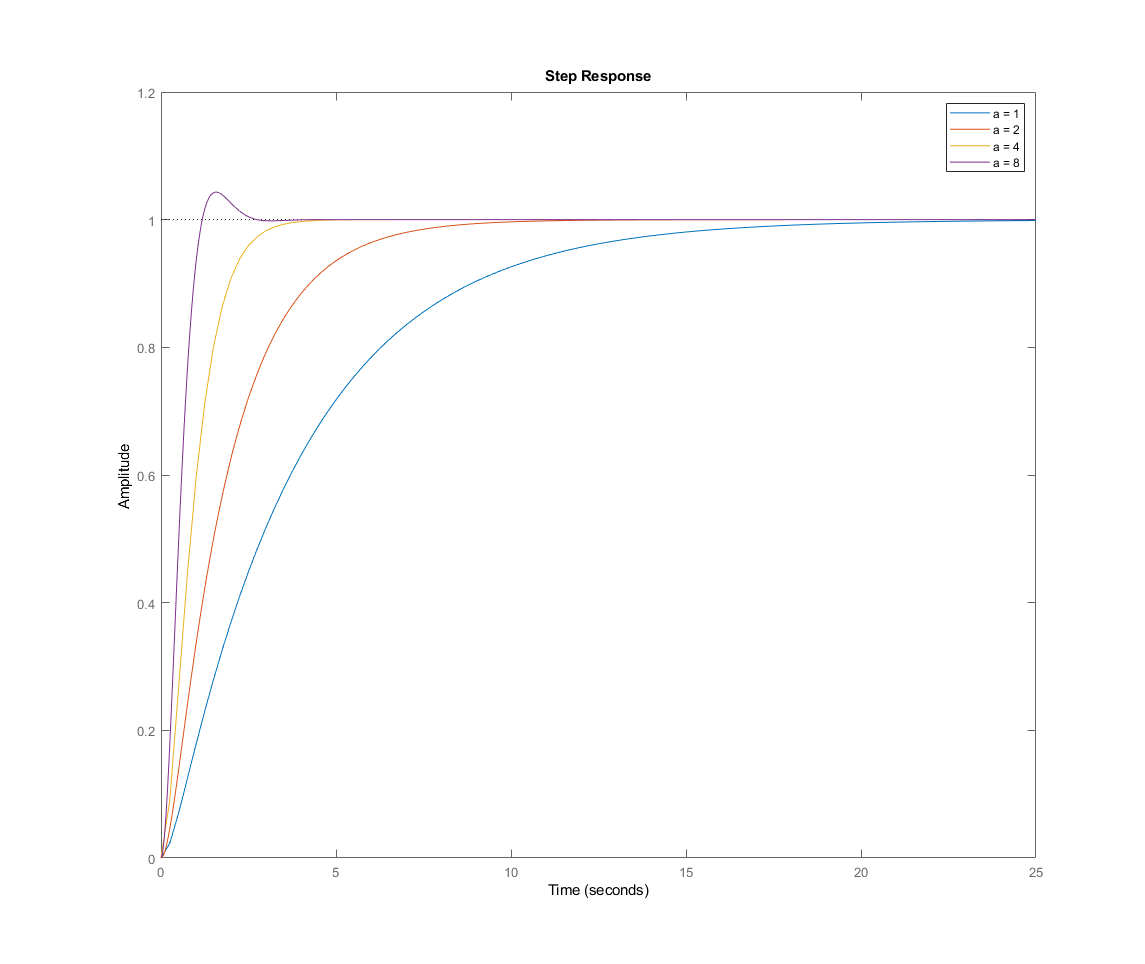
\includegraphics[width=0.49\linewidth]
                {inc/q1fig1.png}}
        \subfloat[Corrosponding Pole/Zero Map]{
                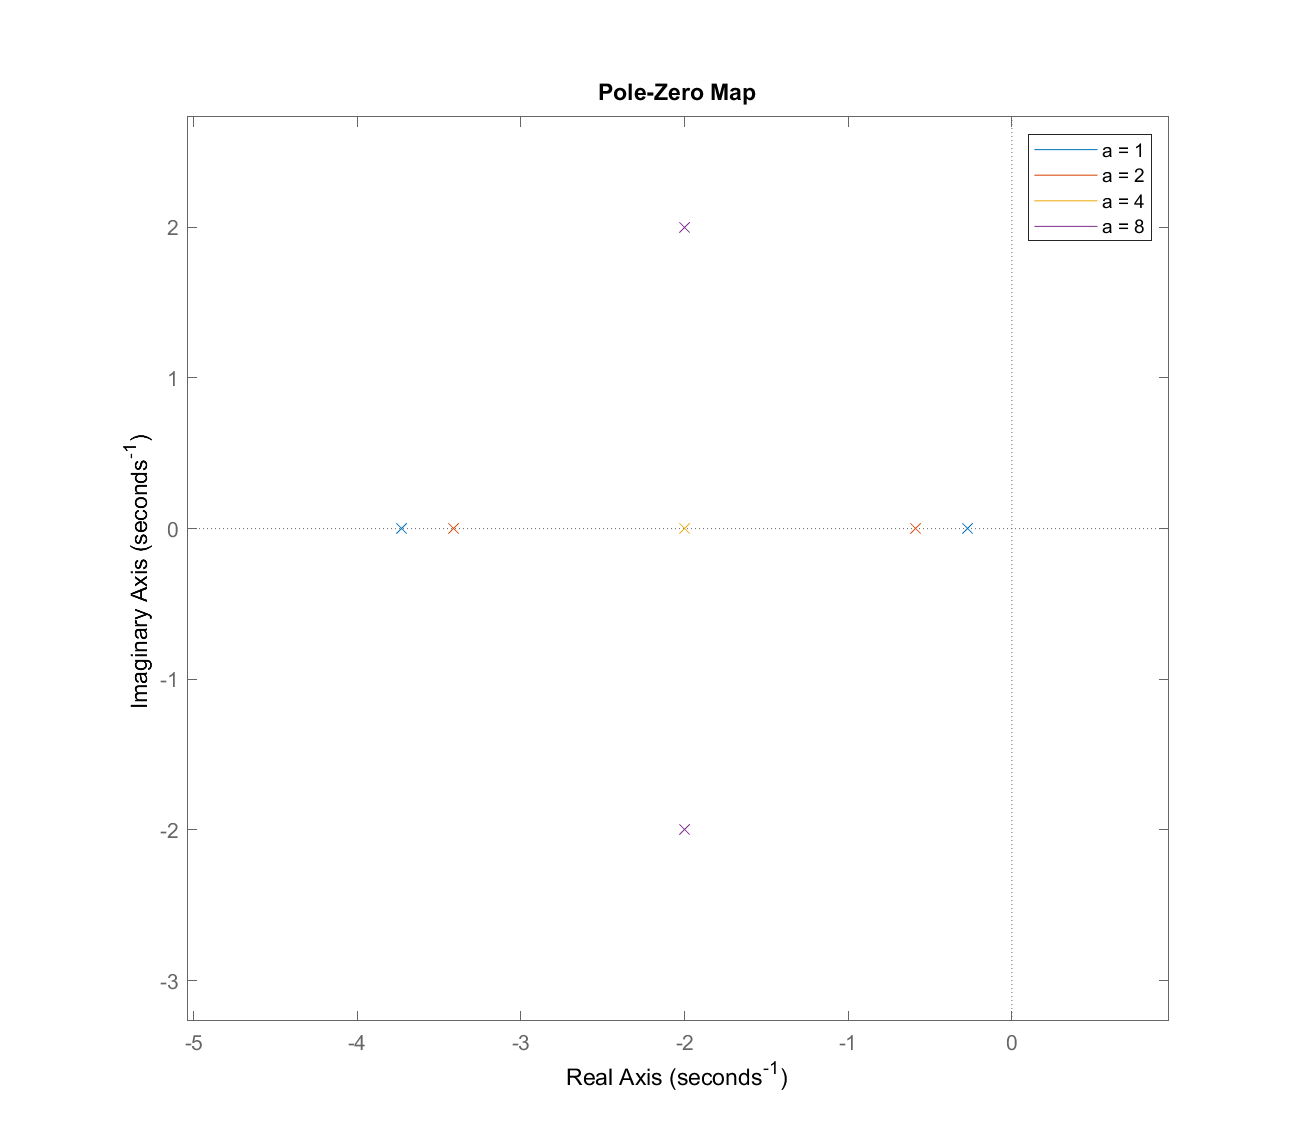
\includegraphics[width=0.49\linewidth]
                {inc/q1fig2.png}}
\caption{$\frac{O}{I} = \frac{a}{s^2 + 4s + a} $}
\end{figure}

\begin{center}
        \begin{tabular}{ll}
                \begin{tabular}[c]{@{}l@{}}
                        For A = 1:\\ 
                        T1 = 3.732051 T2 = 0.267949\\ 
                        T = 1.000000\\ 
                        Ts = 14.878894\\ \\ 
                        
                        For A = 2:\\ 
                        T1 = 1.707107 T2 = 0.292893\\ 
                        T = 0.707107\\ 
                        Ts = 6.999617
                \end{tabular} & \hspace{32pt}  
                \begin{tabular}[c]{@{}l@{}}
                        For A = 4:\\ 
                        T1 = 0.500000 T2 = 0.500000\\ 
                        T = 0.500000\\ 
                        Ts = 2.916978\\ \\ 
                        
                        For A = 8:\\ 
                        T1 = 0.250000 T2 = 0.250000\\ 
                        T = 0.250000\\ 
                        Ts = 2.108152
                \end{tabular}
        \end{tabular}\\
        \vspace{16pt}
        \matlab output
\end{center}

Time constants were calculated via the values given by the damp function (${\omega_{N},\;\zeta}$). \\
$$\tau_{n} = \frac{1}{\omega_{N}{\cdot}\zeta}$$
$$\tau = \sqrt{\tau_{1}{\cdot}\tau_{2}}$$

\newpage
\section*{Question 2}
\begin{enumerate}[label=\alph*)]
        \item  
        \begin{figure}[h]
                \centering
                        \subfloat[]{
                                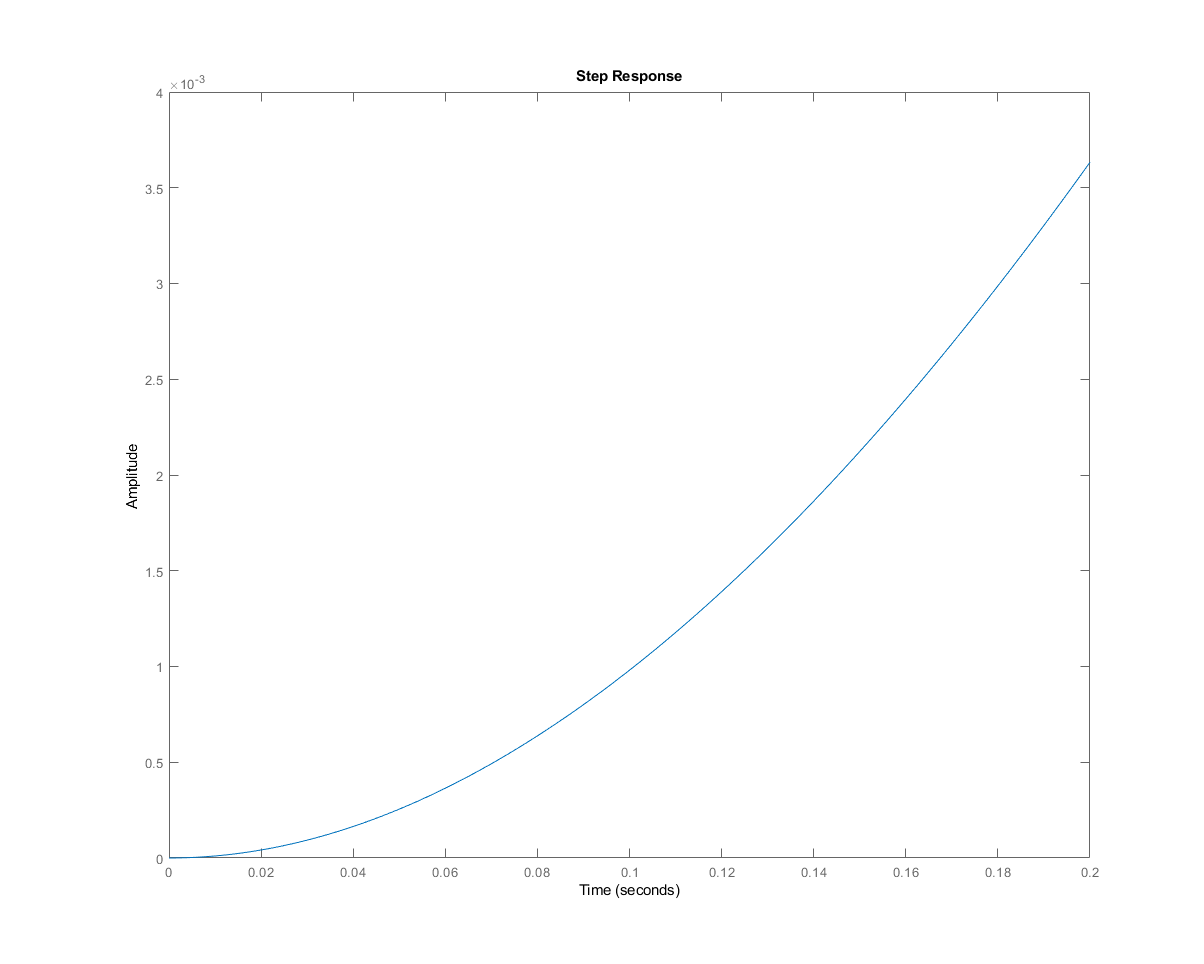
\includegraphics[width=0.49\linewidth]
                                {inc/q2afig1}}
                        \subfloat[]{
                                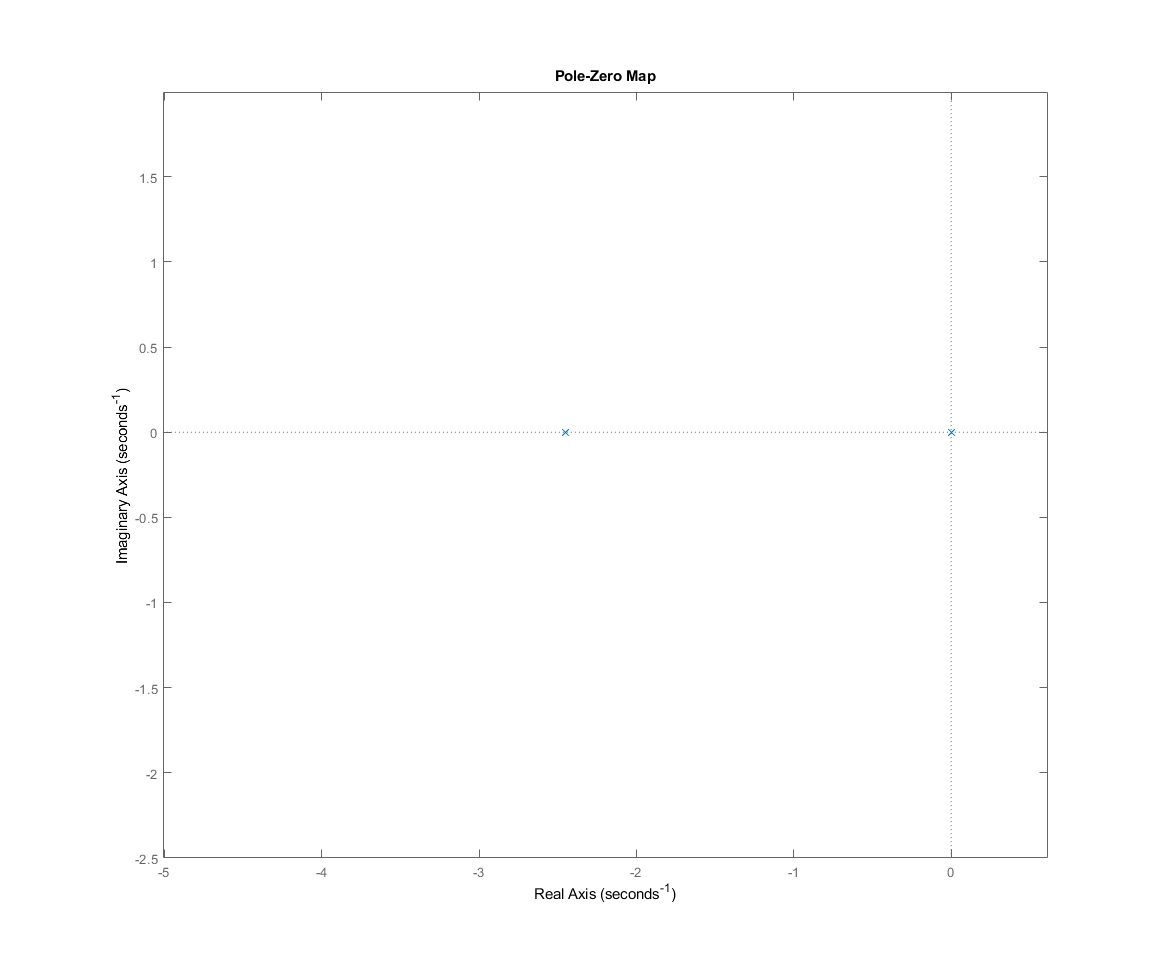
\includegraphics[width=0.49\linewidth]
                                {inc/q2afig2}}
                \caption{}
                \end{figure} 

        Figure 2 shows that step response increases without bounds. This is however to be expected as its the angular displacement of the motor's shaft. Its initial curve shows change but is evened out as it meets max angular velocity.

        \item  
        \begin{figure}[h]
        \centering
                \subfloat[]{
                        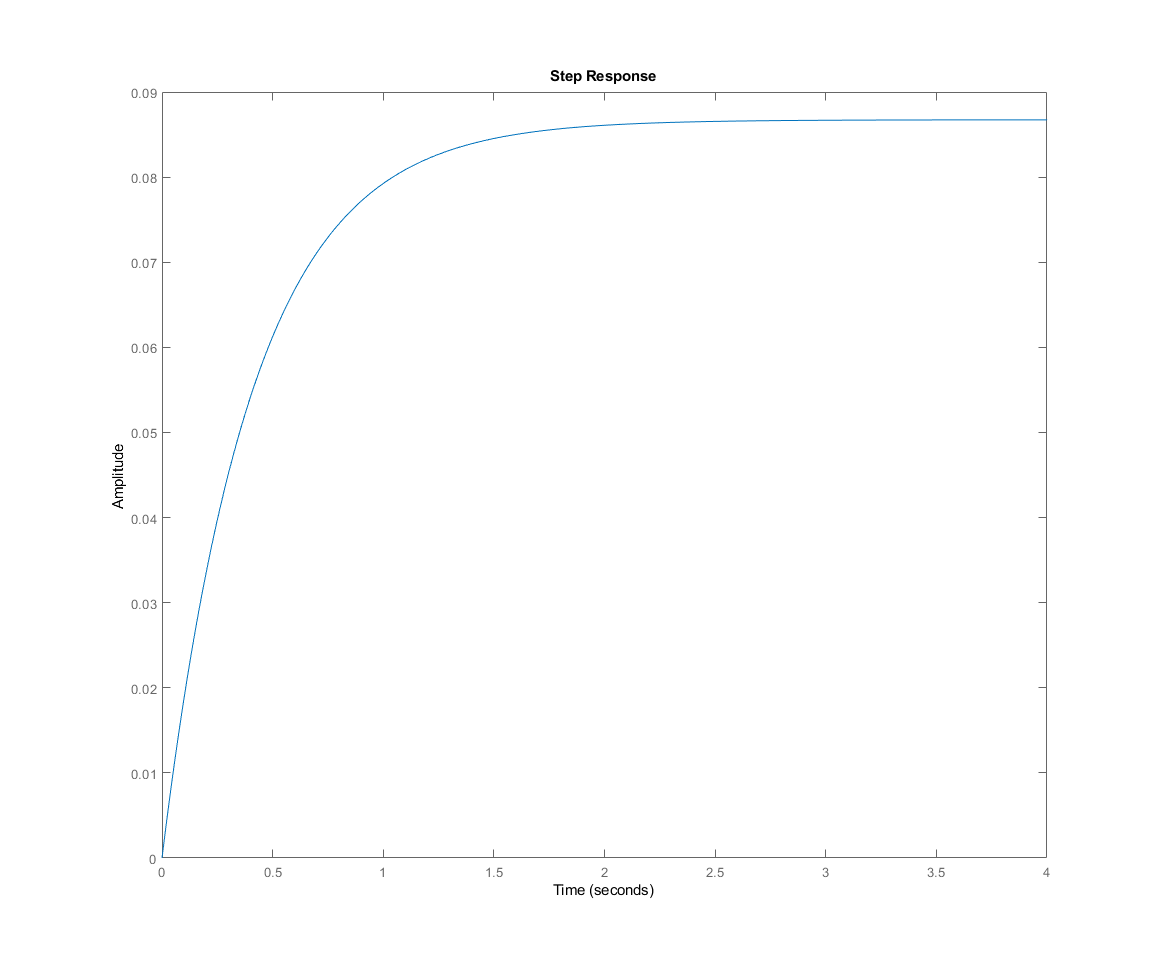
\includegraphics[width=0.49\linewidth]
                        {inc/q2bfig1}}
                \subfloat[]{
                        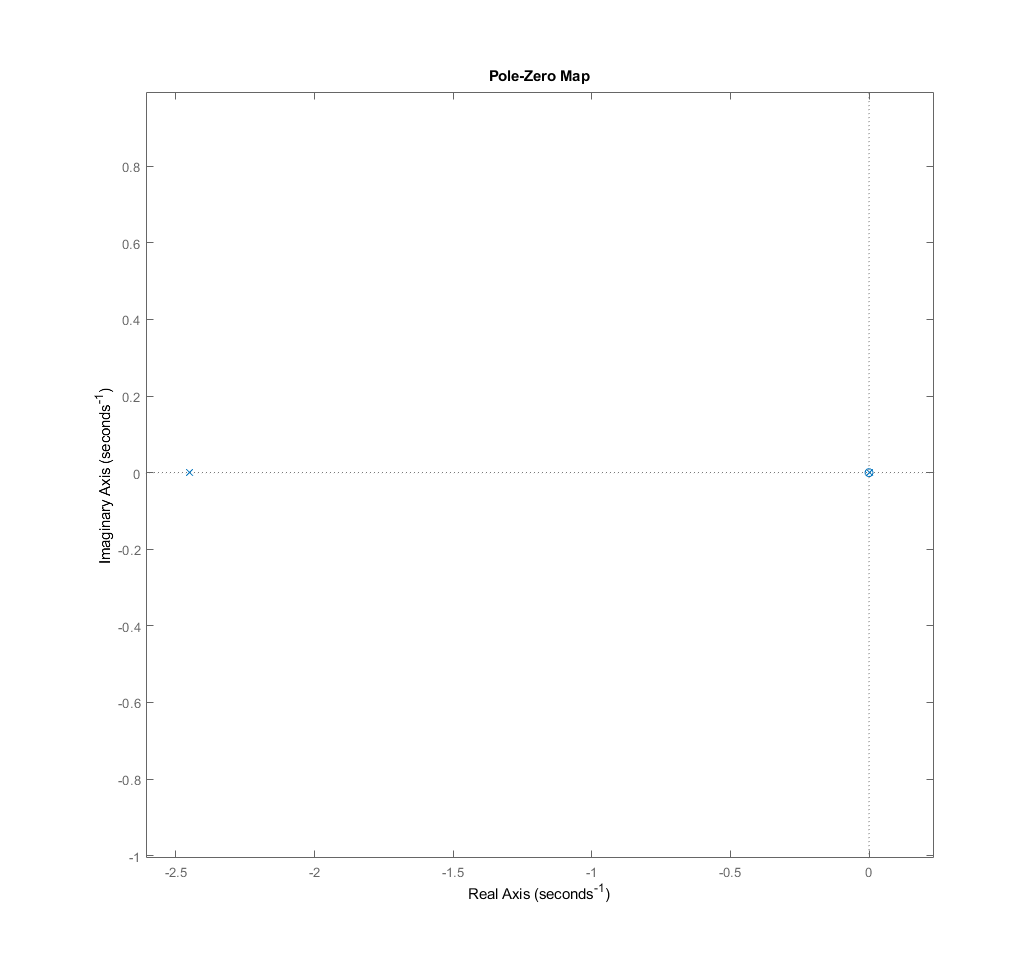
\includegraphics[width=0.49\linewidth]
                        {inc/q2bfig2}}
        \caption{}
        \end{figure} 

        Figure 3 shows the step response of the angular velocity, which is seen to reach a max value (steady state).
\end{enumerate}

\newpage
\section*{Question 3}
\begin{figure}[h]
        \centering
                \subfloat[]{
                        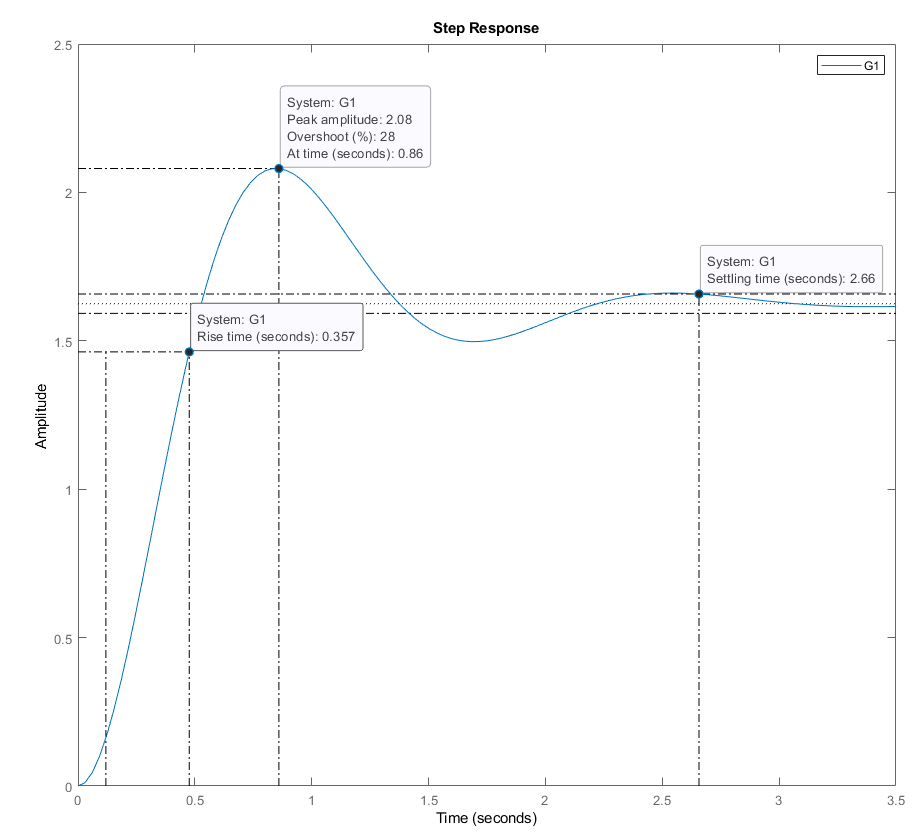
\includegraphics[width=0.3\linewidth]
                        {inc/q3G1}}
                \subfloat[]{
                        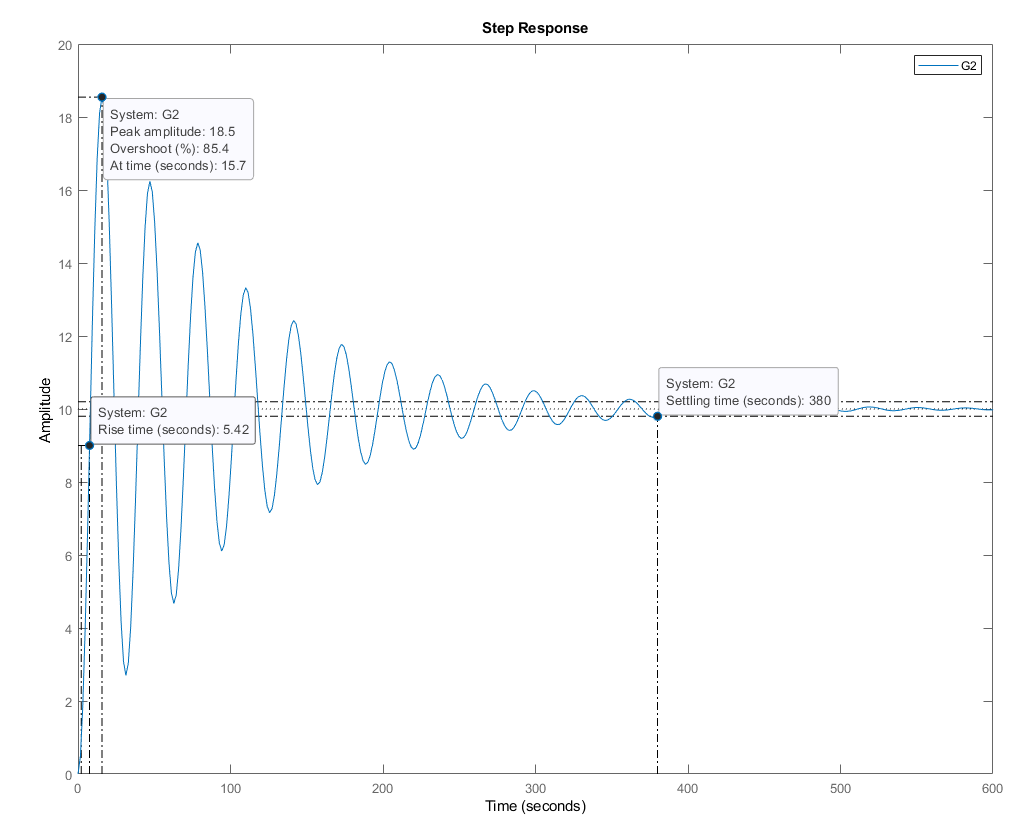
\includegraphics[width=0.3\linewidth]
                        {inc/q3G2}}
                \subfloat[]{
                        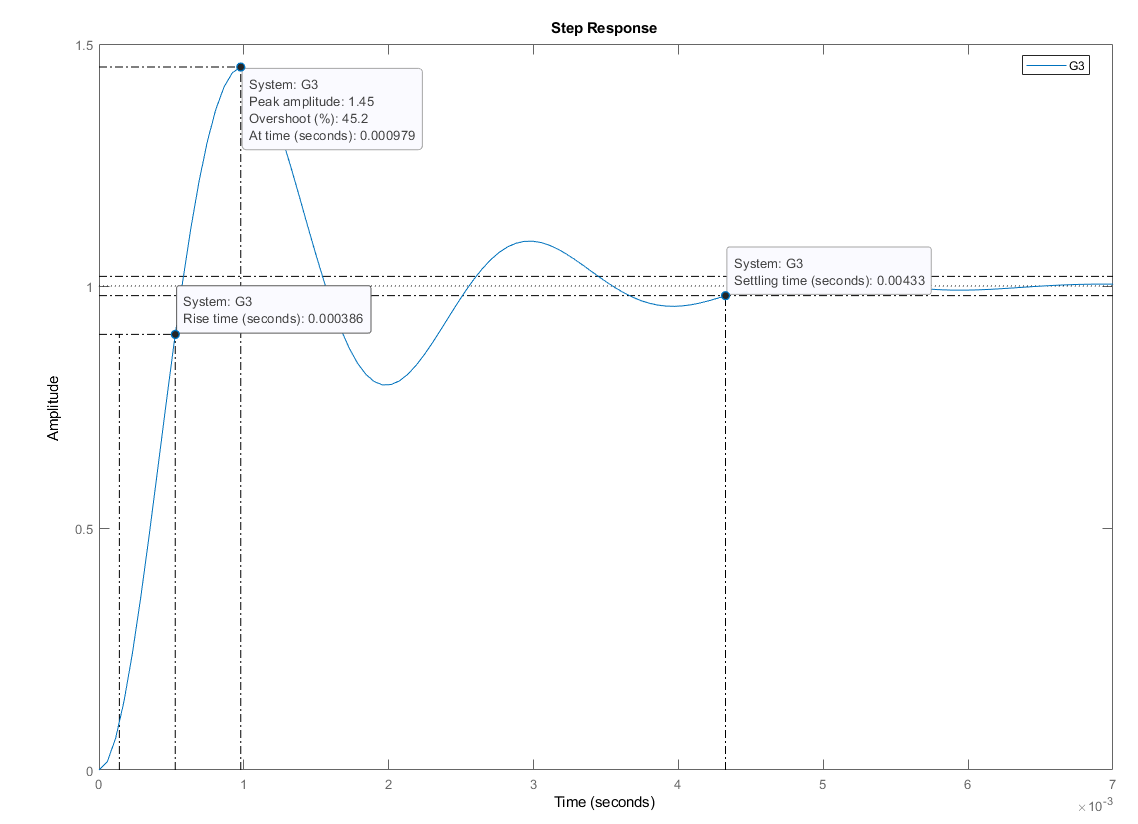
\includegraphics[width=0.3\linewidth]
                        {inc/q3G3}}
        \caption{}
\end{figure} 

\begin{verbatim}
G_1(s): Z=0.375000, Wn=4.000000,    Ts=2.657041,   Tp=0.859632,  Tr=0.356904, OS=28.025548 

G_2(s): Z=0.050000, Wn=0.200000,    Ts=380.016288, Tp=15.707963, Tr=5.416048, OS=85.446128 

G_3(s): Z=0.244567, Wn=3271.085447, Ts=0.004325,   Tp=0.000979,  Tr=0.000386, OS=45.241508 
\end{verbatim}

Figure 4 shows each of the of three systems: 

$$G_{1}(s)=\frac{26}{s^2 + 3s + 16}$$
$$G_{2}(s)=\frac{0.4}{s^2 + 0.02 + 0.04}$$
$$G_{3}(s)=\frac{1.07{\times}10^7}{s^2 + 1.6{\times}10^3s + 1.07{\times}10^7}$$

With the rise, settling and peak/overshoot data marked at their occurrence. The verbatim text shows the output of the \matlab script's calculated values; ($\zeta,\; \omega_{n},\; \tau_{s},\; \tau_{p},\; \tau_{r},\; \%OS$)

\section*{Question 4}
\begin{figure}[h]
        \centering
                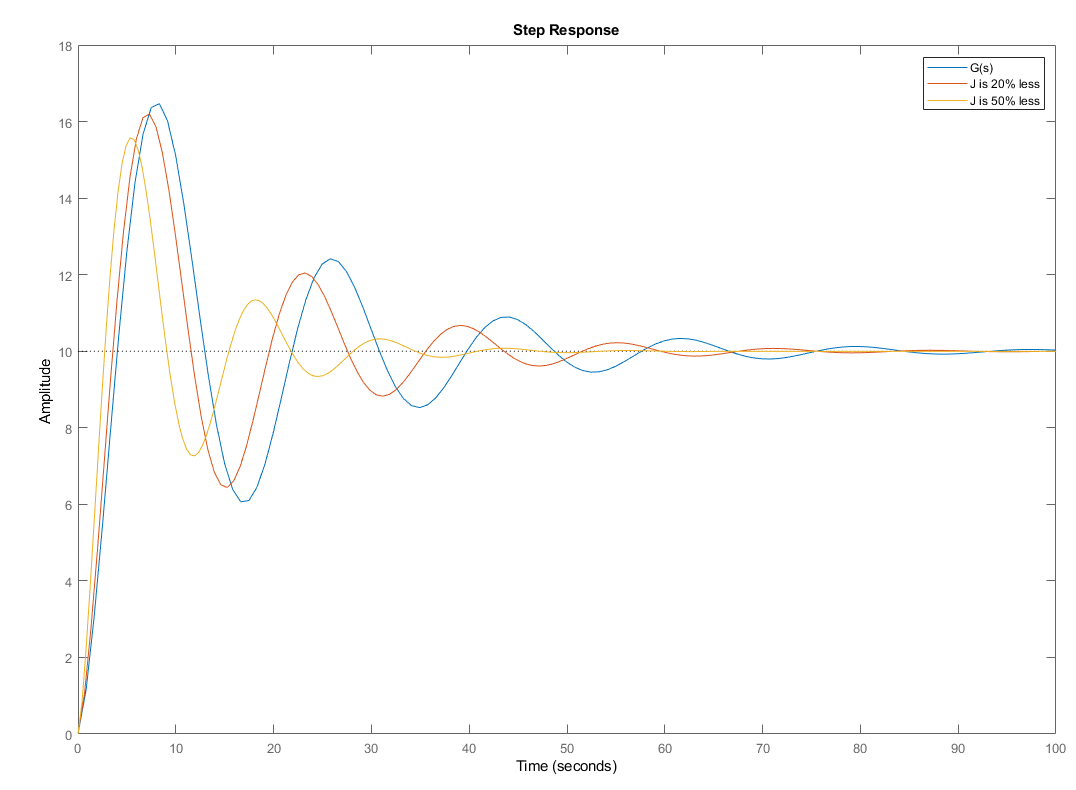
\includegraphics[width=\linewidth]
                {inc/q4fig}
        \caption{$G(s) = \frac{\Theta(s)}{\Theta_{d}(s)}$}
\end{figure} 

Figure 5 plots the output of a 10$^\circ$ step input to G(s), compared with the reduction of J by 20\% and 50\% and the effect on the settling time displayed.

\matlab computed the TF to be equal to, $\frac{\Theta(s)}{\Theta_{d}(s)} = \frac{1.08e09 s + 1.08e09}{1.08e09 s^3 + 8.64e09 s^2 + 1.08e09 s + 1.08e09}$ 

\newpage
\section*{Question 5}
\begin{enumerate}[label=\alph*)]
        \item  
        \begin{figure}[h]
                \centering
                        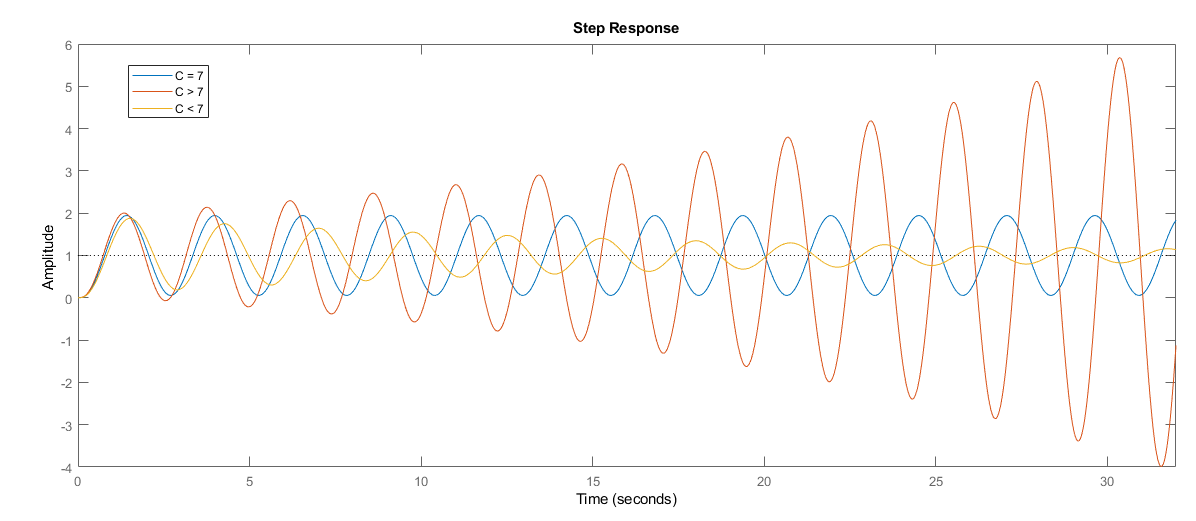
\includegraphics[width=\linewidth]
                        {inc/q5a}
                \caption{}
        \end{figure} 
        \begin{verbatim}
                MatLab Output: Minimum series gain > 7.000000
        \end{verbatim}

Using a search loop iterating the value of C, the gain value that gives a marginally stable system was found to be 7. 

$\therefore$ the system is unstable at $C > 7$

Figure 6 shows step response for the foundry case C=7 and either side.

        \item  
        \begin{figure}[h]
                \centering
                \subfloat[]{
                        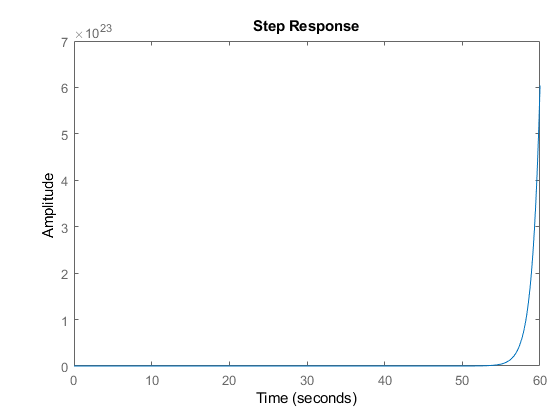
\includegraphics[width=0.49\linewidth]
                        {inc/q5bfig1}}
                \subfloat[]{
                        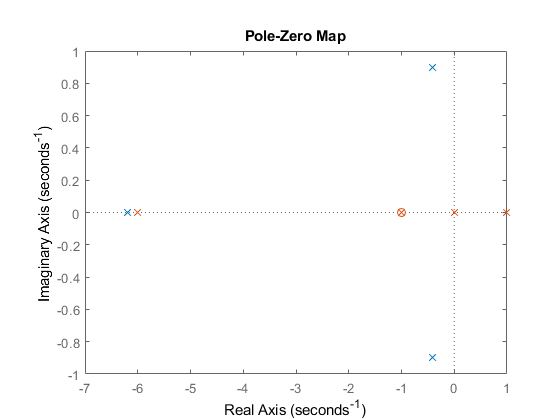
\includegraphics[width=0.49\linewidth]
                        {inc/q5bfig2}}
                \caption{}
        \end{figure} 
\end{enumerate}

Using a lead-lag controller $C(\frac{s-z}{s-p}) = 0.01(\frac{s+1}{s-1})$ to place a pole at positive 1 with a lower steady state gain than (a): 7 compared to -0.01).

\newpage
\section*{Appendices}
\subsection*{Task 1}
\lstinputlisting{q1.m}
\subsection*{Task 2}
\lstinputlisting{q2.m}
\newpage
\subsection*{Task 3}
\lstinputlisting{q3.m}
\subsection*{Task 4}
\lstinputlisting{q4.m}
\newpage
\subsection*{Task 5}
\lstinputlisting{q5.m}
\end{document}
